% !TEX root = ../entropy.tex

\section{Method}%
\label{sec:method}


\subsection{Dataset description}
\label{sub:dataset_description}

We use data from Money Dashboard (MDB), a financial management app that allows
its users to link accounts from different banks to obtain an integrated view of
their
finances.\footnote{\href{https://www.moneydashboard.com}{https://www.moneydashboard.com}.}
The dataset contains more than 500 million transactions made between 2012 and
June 2020 by about 250,000 users, and provides information such as date,
amount, and description about the transaction as well as account and user-level
information.

The main advantages of the data for the study of consumer financial behaviour
are its high frequency, that it is automatically collected and updated and thus
less prone to errors and unaffected by biases that bedevil survey measures, and
that it offers a view of consumers' entire financial life across all their
accounts, rather than just a view of their accounts held at a single bank,
provided they added all their accounts to MDB. The main limitation is the
non-representativeness of the sample relative to the population as a whole.
Financial management apps are known to be used disproportionally by men,
younger people, and people of higher socioeconomic status
\citep{carlin2019generational}. Also, as pointed out in
\citet{gelman2014harnessing}, a willingness to share financial information with
a third party might not only select on demographic characteristics, but also
for an increased need for financial management or a higher degree of financial
sophistication. Because our analysis does not rely on representativeness, we do
not address this.\footnote{For an example of how re-weighing can be used to
mitigate the non-representative issue, see \citet{bourquin2020effects}.}


\subsection{Preprocessing and sample selection}%
\label{sub:preprocessing_and_sample_selection}

We restrict our sample to users for whom we can observe a regular income, can
be reasonably sure that they have added all their bank account to MDB, and for
whom we observe at least six months of data. Table~\ref{tab:selection}
summarises the sample selection steps we applied to a 1 percent sample of the
raw data, associated data losses, and the size of our final sample. A detailed
description of the entire data cleaning and selection process is provided in
Appendix~\ref{sec:data}.

\begin{table}[H]
\caption{Sample selection}\label{tab:selection}
\begin{tabular}{lrrrr}
\toprule
                                                 &  Users & Accounts & Transactions & Value (\pounds M) \\
\midrule
                                      Raw sample & 24,163 &  123,625 &   59,647,019 &          11,209.7 \\
                       At least 6 months of data & 21,508 &  117,000 &   59,088,076 &          11,116.8 \\
                               No missing months & 18,550 &   98,513 &   51,252,412 &           9,606.4 \\
                      Account balances available & 14,714 &   85,590 &   44,163,629 &           8,618.7 \\
At least 5 debits totalling \pounds200 per month & 12,296 &   70,981 &   38,618,825 &           7,469.7 \\
                    At least one current account & 12,148 &   70,366 &   38,280,116 &           7,421.9 \\
            Income in 2/3 of all observed months &  9,963 &   60,151 &   33,270,455 &           6,490.2 \\
 Yearly income between \pounds5k and \pounds200k &  6,716 &   36,829 &   21,460,727 &           3,677.9 \\
            No more than 10 accounts in any year &  6,169 &   26,999 &   18,241,355 &           2,855.1 \\
      Debits of less than \pounds100k each month &  5,760 &   24,486 &   16,409,561 &           1,998.7 \\
                                    Final sample &  5,760 &   24,486 &   16,409,561 &           1,998.7 \\
\bottomrule
\end{tabular}

\end{table}


\subsection{Variable description}%
\label{sub:dependent_variable}

Our outcome variable is a binary indicator for whether or not a user has made
any payments into their savings accounts in a given month. We classify as
payments into savings accounts all savings account credits of \pounds5 or more
that are not identified as interest payments or automated "save the change"
transfers. While standing order transactions are unlikely to be related to
entropy in the short-run, we do not exclude such transactions since, best we
can tell, the only account for a small fraction of total transactions.

Our variable of interest is the degree of chaos of an individual's lifestyle.
We ...

--todo--


\subsection{Independent variable}%
\label{sub:independent_variable}

Spending entropy:

\begin{itemize}

    \item We calculate spending entropy using the Shannon entropy
        \textit{H}\citep{shannon1948mathematical}, defined as

        \begin{equation}
            H = -\sum{p_i}log(p_i),
        \end{equation}

    where $p_i$ is the probability that an individual makes a purchase in
    spending category $i$, and $log$ is the base 2 logarithm. The measure can
    broadly be interpreted as the degree to which an individual's spending
    pattern is predictable, whith a higher score indicating less
    predictability.

    \item To calculate individual entropy scores, we group spending into 9
        spending categories (SC), based on the classification used by Lloyds
        Banking Group as discussed in \citet{muggleton2020evidence}.
        Transactions included in the calculation are those classified as one of
        those spending categories that are debits and were made either from an
        indivuals current or credit card account.

    \item Also following that paper, when calculating $p_i$ we use additive
        smoothing and add one to the numerator and $N_{SC}$ to the denominator
        to avoid taking logs of zero counts in cases where an individual makes
        no purchases in a given spending category. $p_i$ is thus calculated as

        \begin{equation}
            p_i = \frac{\text{Count of purchases in $SC_i$} + 1}{\text{Count of
            all purchases} + 9}
        \end{equation}

\end{itemize}

\begin{figure}[H]
    \center \newcommand\width{\textwidth} \caption{Transactions distributions}
    \label{fig:entropy_dist}
    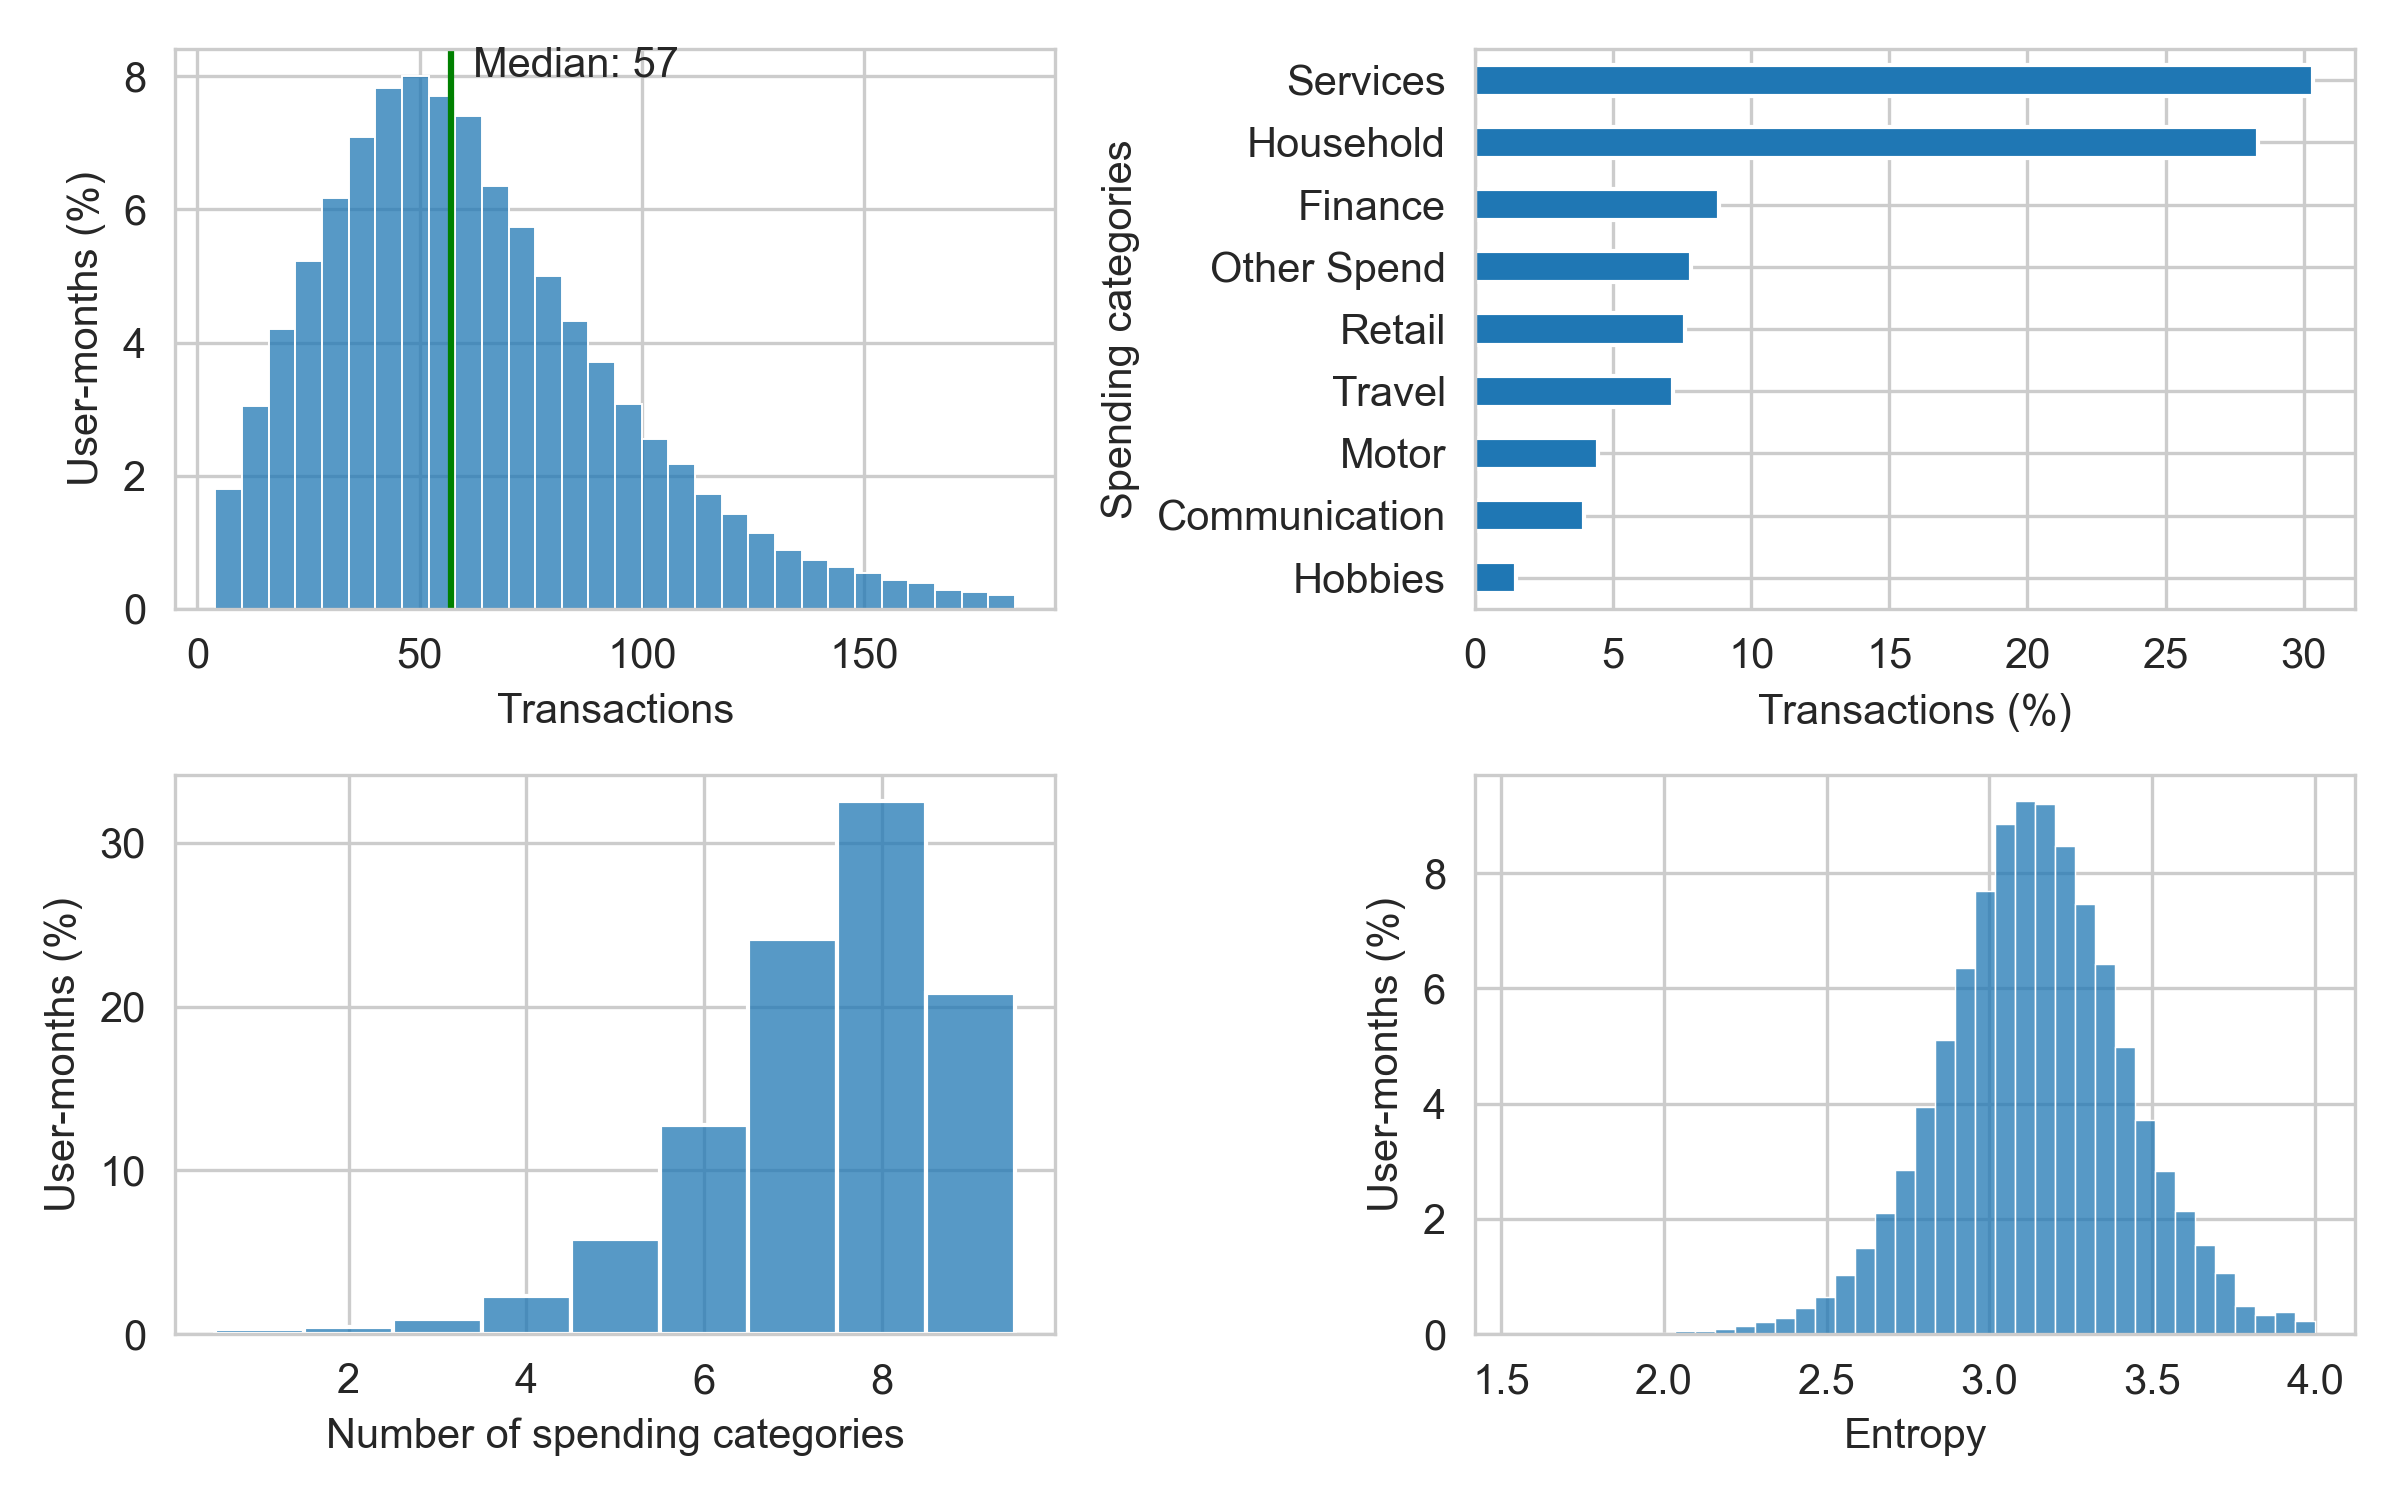
\includegraphics[width=\width]{\figdir/txns_breakdowns_and_entropy.png}
    \fignote{\width}{From top-left to bottom-right: distribution of spending
    transactions per user-month, breakdown of spending transactions into
spending categories; breakdown of number of spending categories spent on in
user-month; distribution of user-month entropy scores.}

\end{figure}

\subsection{Control variables}%
\label{sub:control_variables}

We calculate age as an individual's approximate age at the time of the
transactions, by subtracting a user's year of birth from the year the
transaction took place.


\subsection{Summary statistics}%
\label{sub:summary_statistics}

The four panels in Figure~\ref{fig:sumstats} provide an overview of
demographic characteristics of our sample. It makes clear that Money Dashboard
users are not a representative sample of the UK population: they are
predominantly males in their thirties who live in London or the South East and
are relatively well off (the income distribution is shifted to the right
relative to the UK as a whole).\footnote{To calculate incomes, we broadly
    follow \citet{hacioglu2020distributional} in defining total income as the
sum of earnings, pension income, benefits, and other income.} 

\begin{figure}[H]
    \caption{Demographic characteristics of Money Dashboard users}
    \label{fig:sumstats}
    \begin{center}
        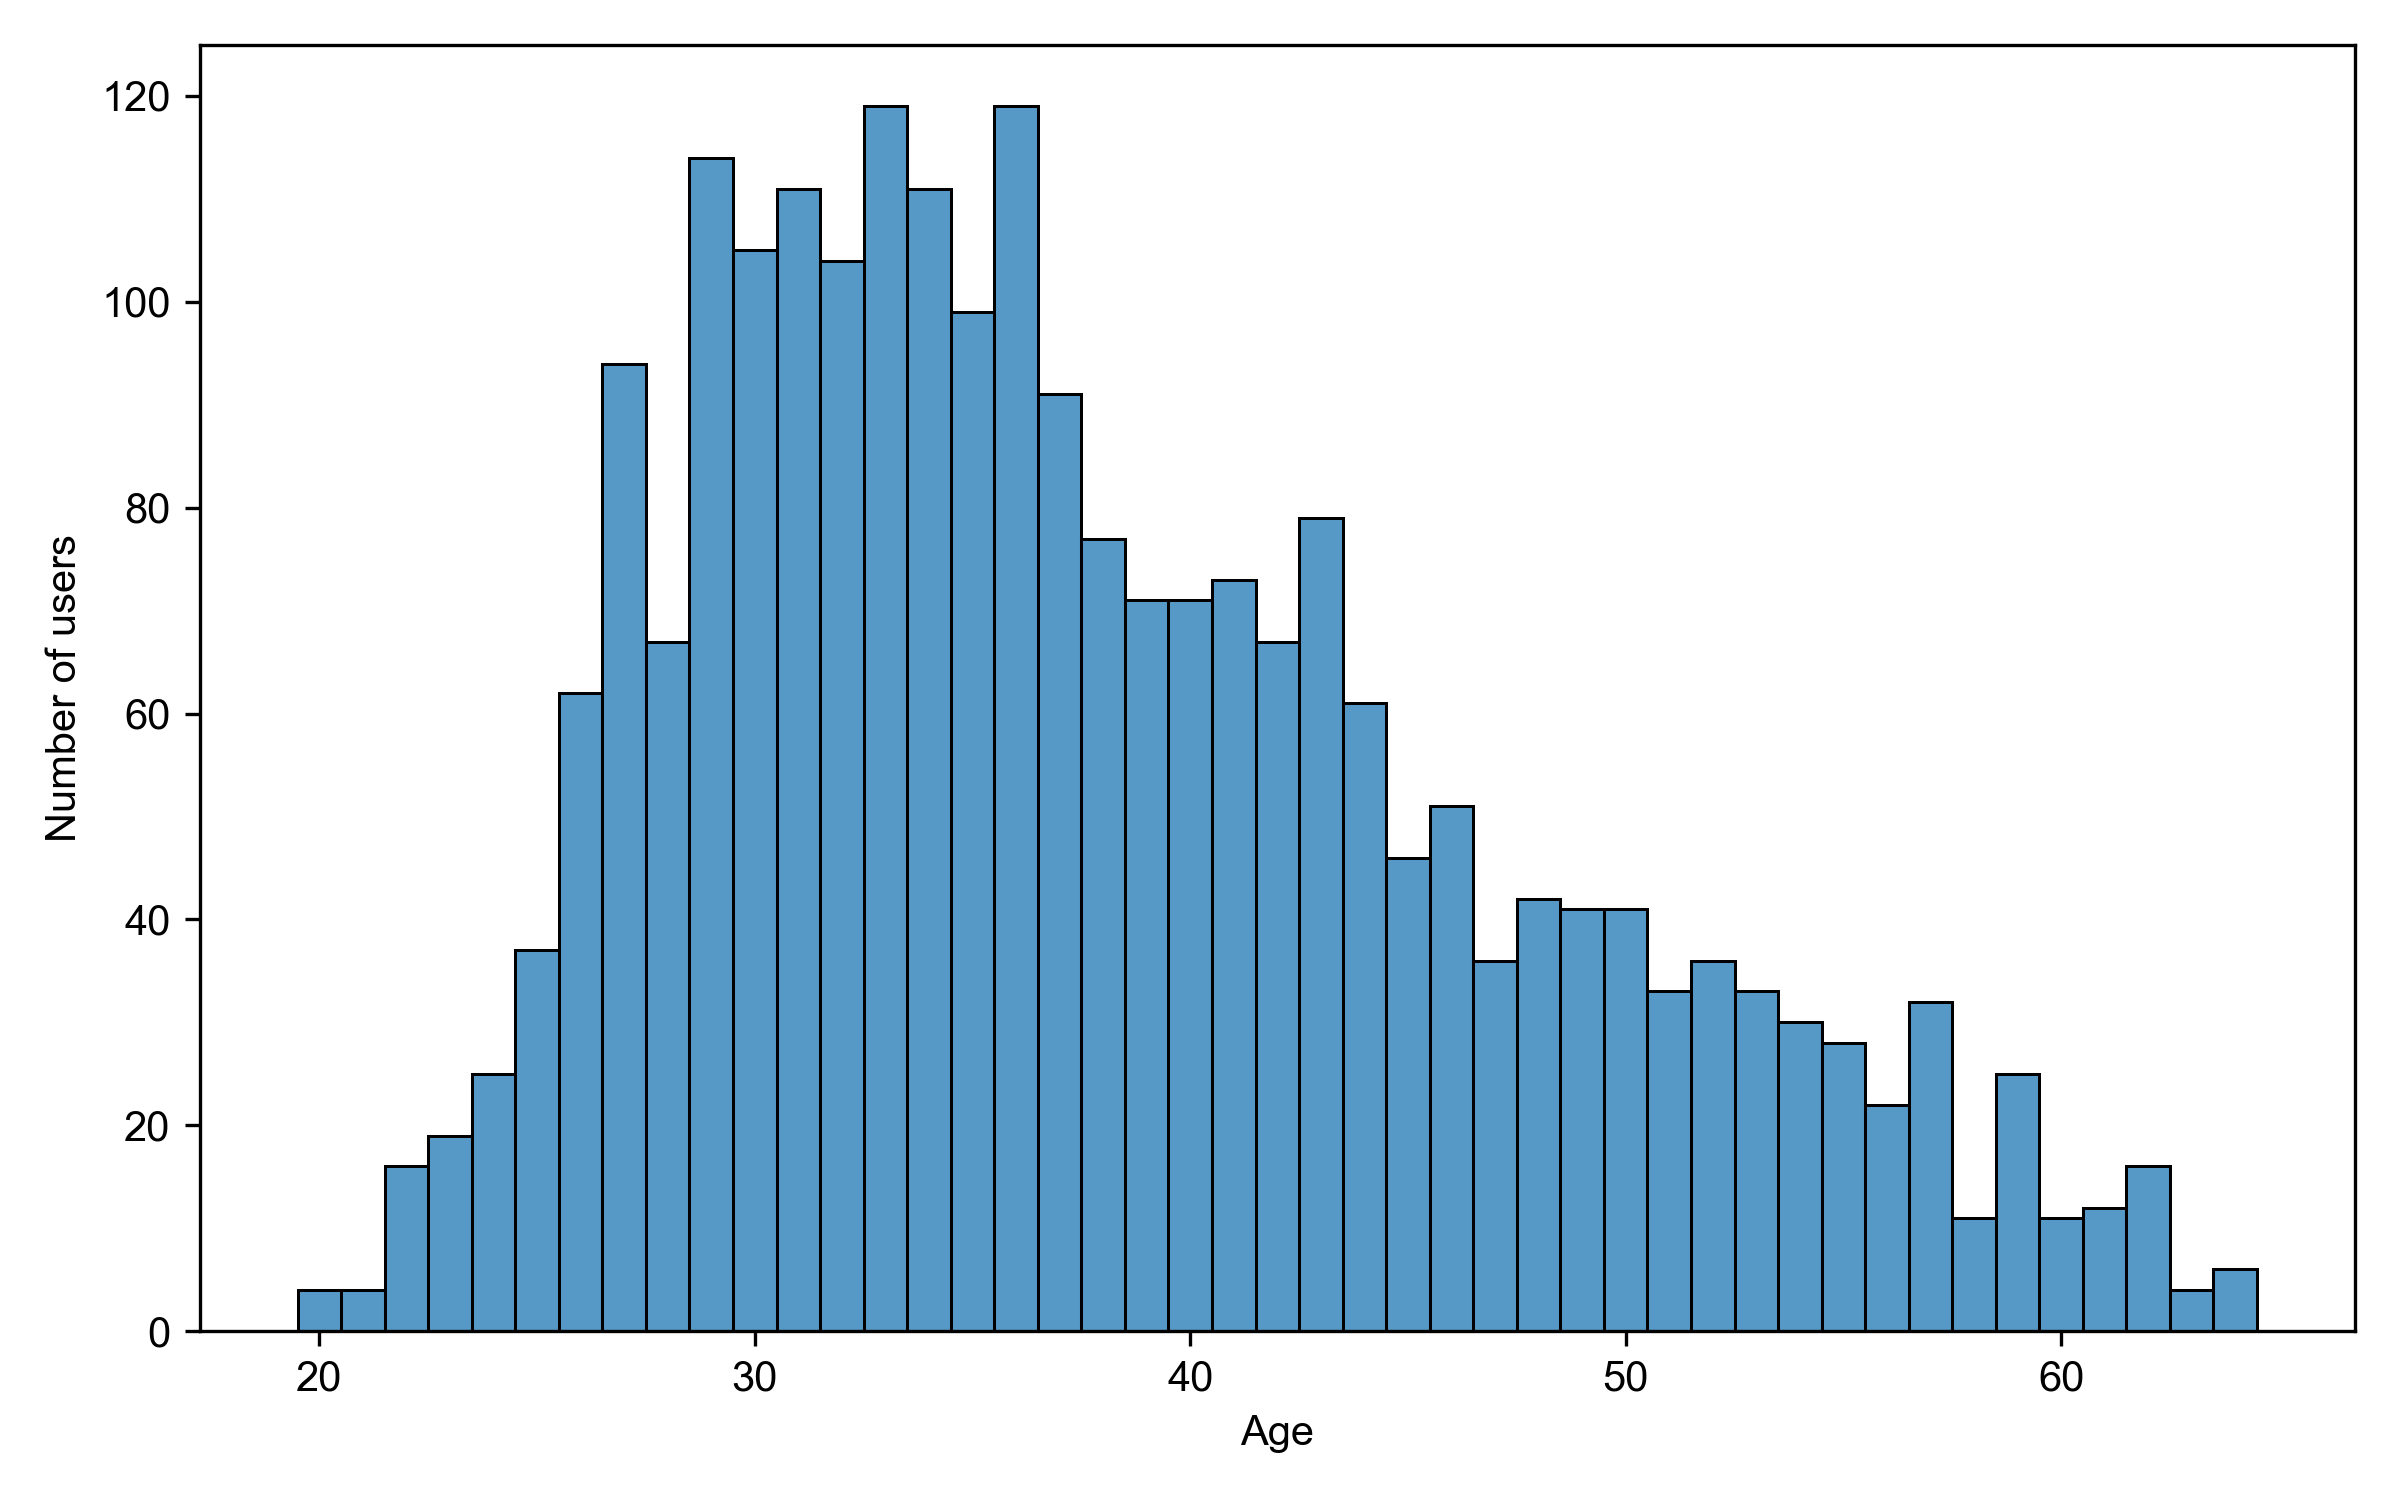
\includegraphics[width=0.49\textwidth]{\figdir/user_age_hist.png}
        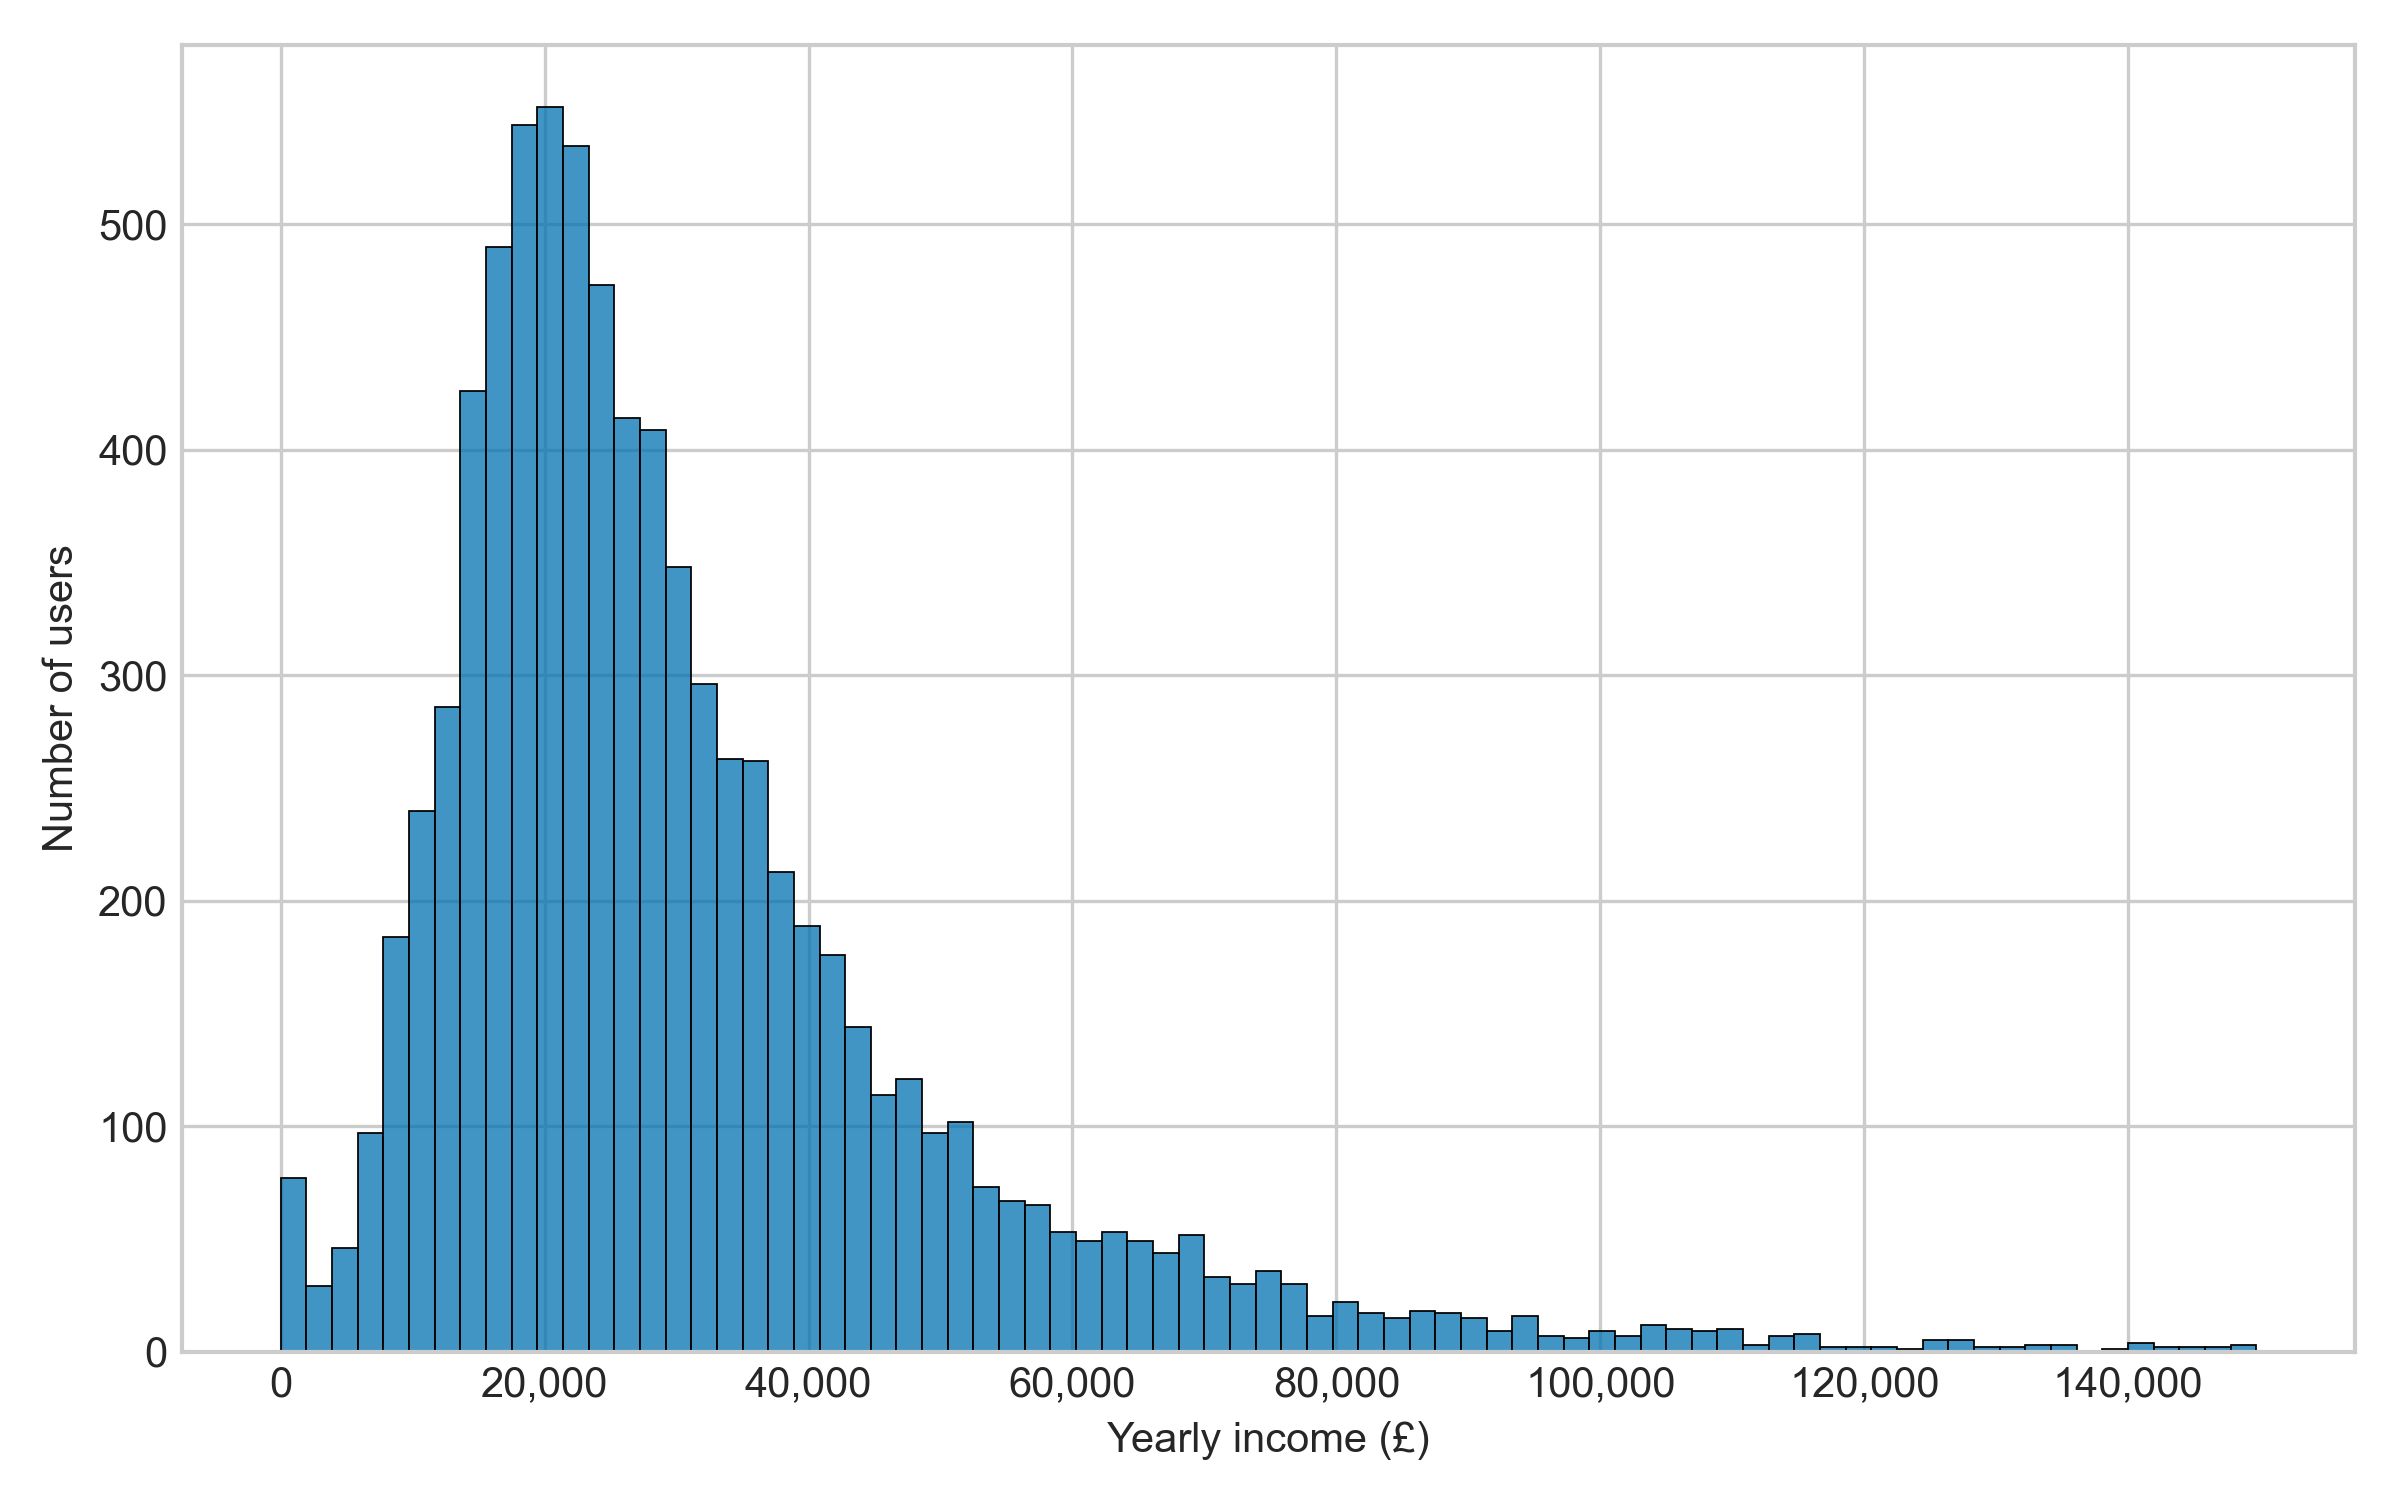
\includegraphics[width=0.49\textwidth]{\figdir/user_income_hist.png}
        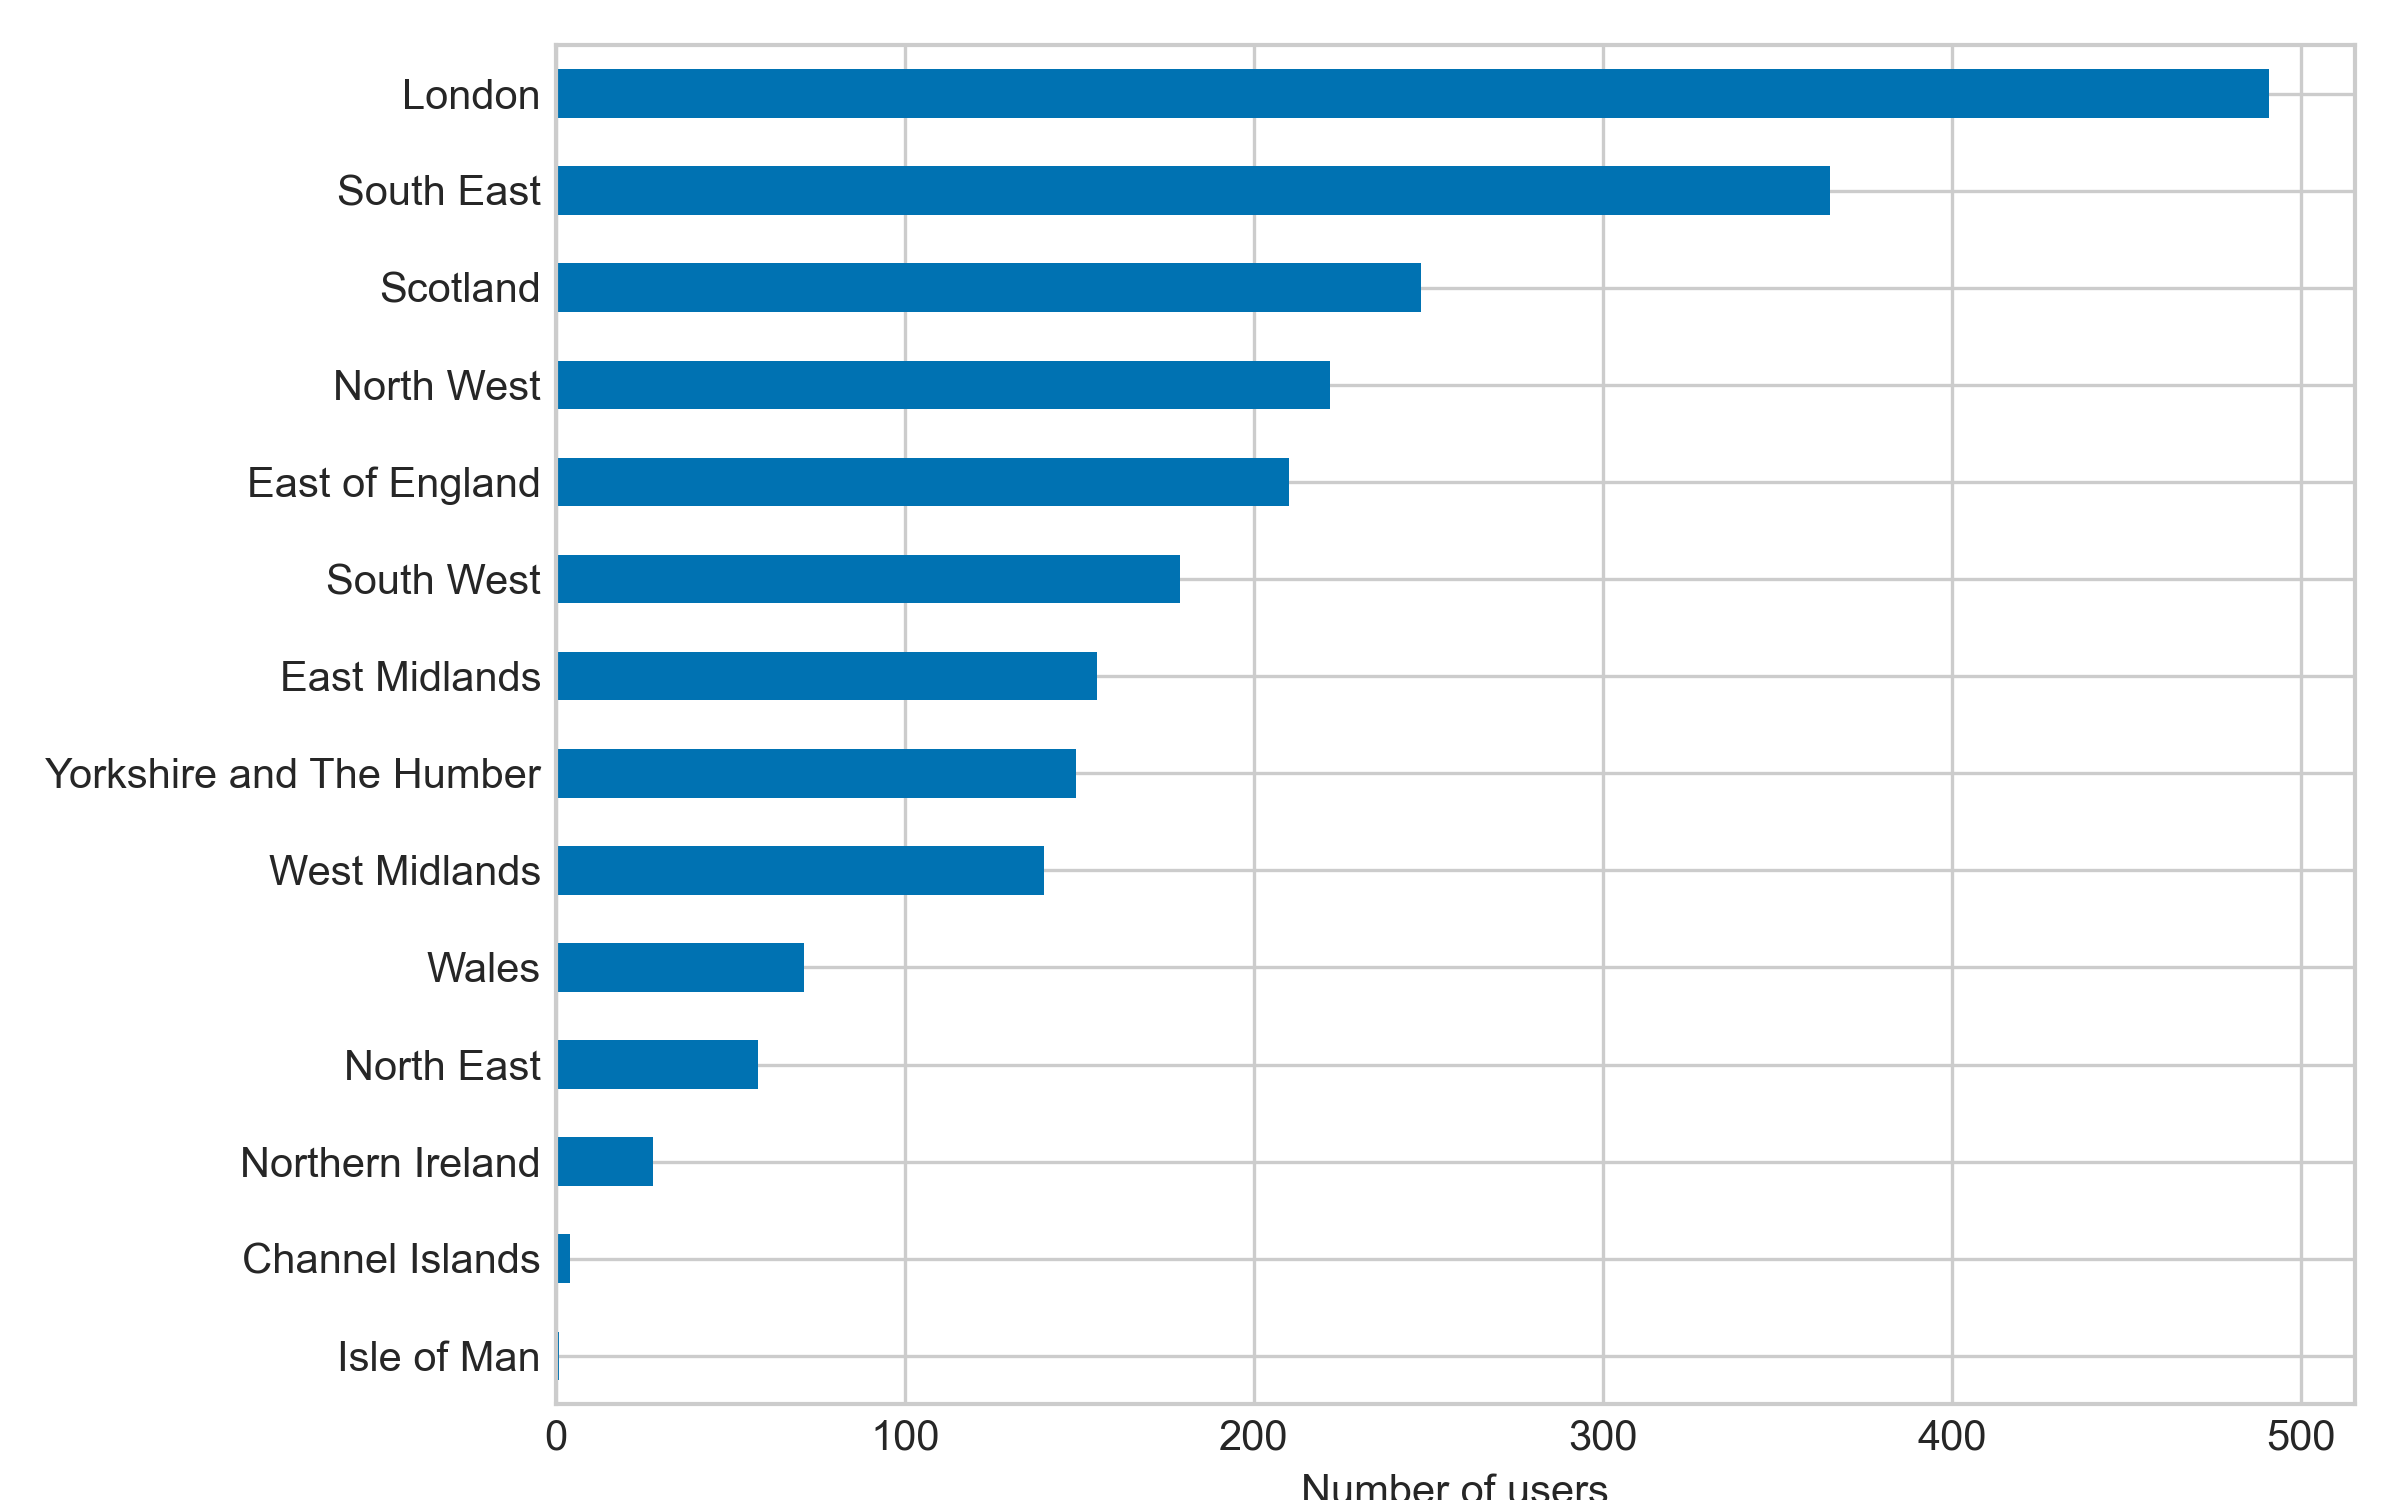
\includegraphics[width=0.49\textwidth]{\figdir/user_region_distr.png}
        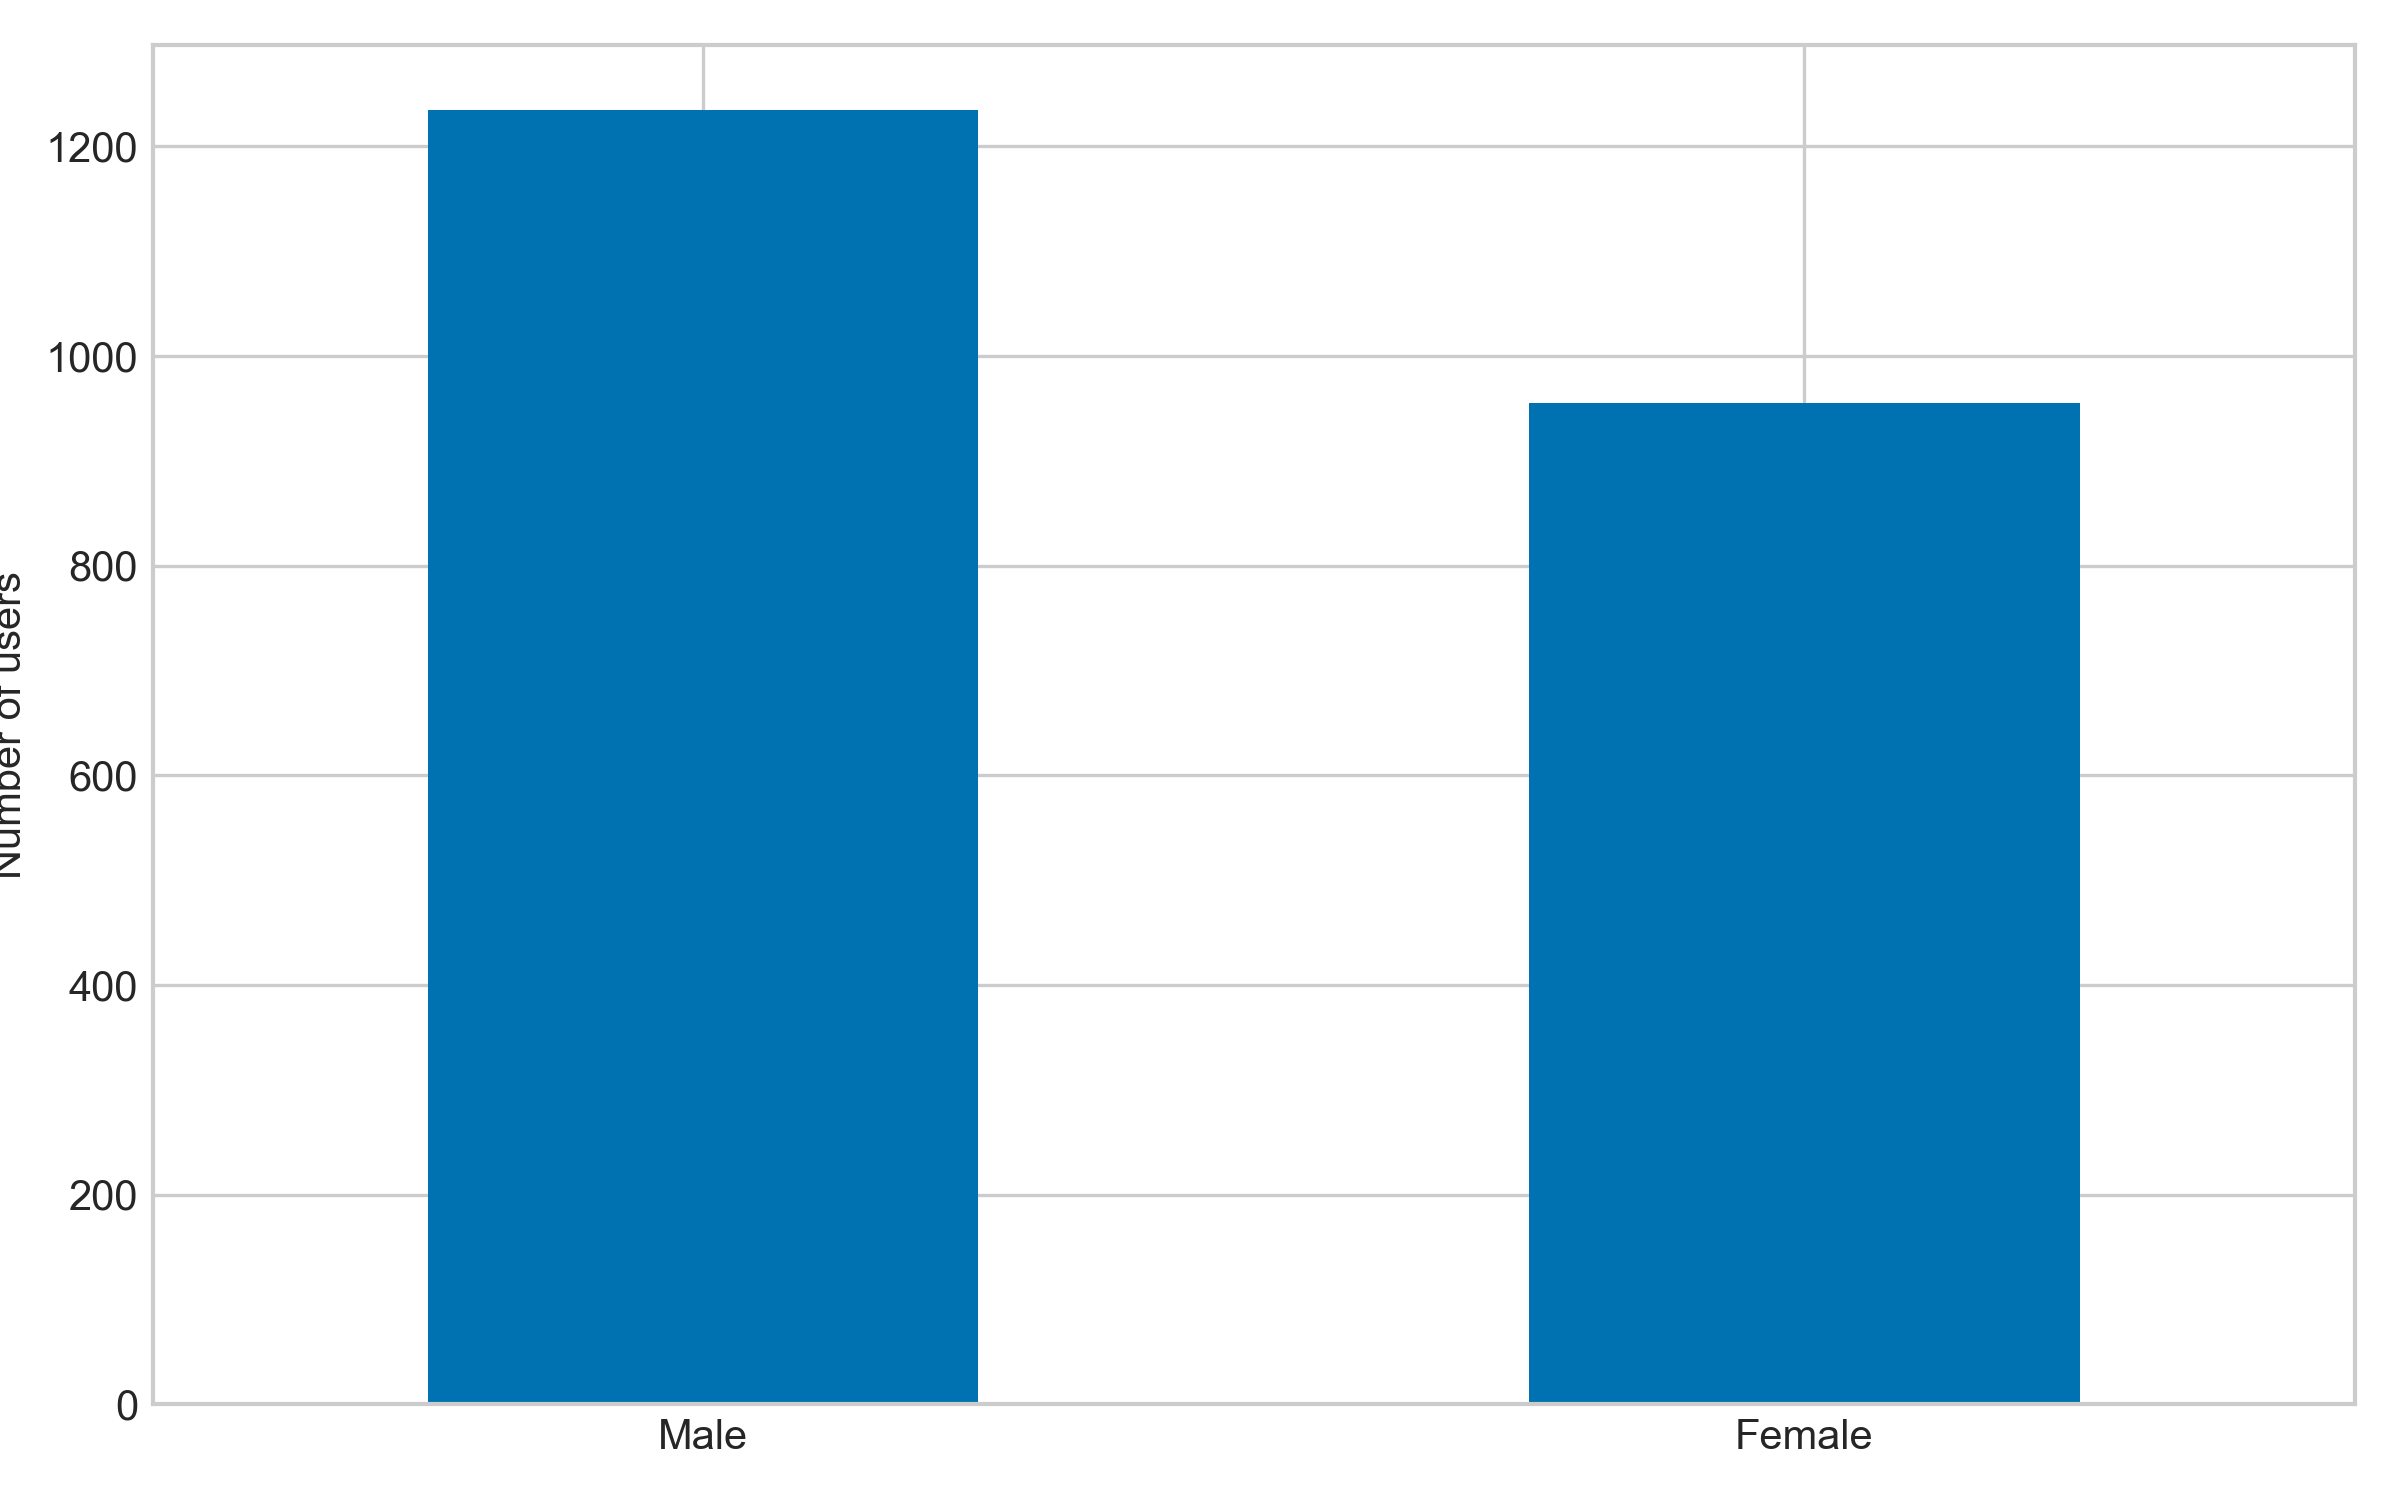
\includegraphics[width=0.49\textwidth]{\figdir/user_gender_distr.png}
    \end{center}
\end{figure}

\begin{table}[H]
\caption{Summary statistics}\label{tab:sumstats}

% Table created by stargazer v.5.2.3 by Marek Hlavac, Social Policy Institute. E-mail: marek.hlavac at gmail.com
% Date and time: Mon, Sep 26, 2022 - 09:41:15
\begin{tabular}{@{\extracolsep{5pt}}lccccccc} 
\\[-1.8ex]\hline 
\hline \\[-1.8ex] 
Statistic & \multicolumn{1}{c}{Mean} & \multicolumn{1}{c}{St. Dev.} & \multicolumn{1}{c}{Min} & \multicolumn{1}{c}{Pctl(25)} & \multicolumn{1}{c}{Median} & \multicolumn{1}{c}{Pctl(75)} & \multicolumn{1}{c}{Max} \\ 
\hline \\[-1.8ex] 
Month income & 2.77 & 2.23 & 0.00 & 1.45 & 2.18 & 3.43 & 13.69 \\ 
Has income in month & 0.98 & 0.13 & 0 & 1 & 1 & 1 & 1 \\ 
Has savings & 0.50 & 0.50 & 0 & 0 & 1 & 1 & 1 \\ 
Month spend & 2.90 & 2.50 & 0.20 & 1.37 & 2.20 & 3.49 & 16.05 \\ 
Age & 35.72 & 9.74 & 18 & 28 & 34 & 42 & 65 \\ 
Female & 0.43 & 0.49 & 0 & 0 & 0 & 1 & 1 \\ 
Urban & 0.85 & 0.36 & 0 & 1 & 1 & 1 & 1 \\ 
Unique categories (9) & 7.84 & 1.05 & 1 & 7 & 8 & 9 & 9 \\ 
Unique categories (48) & 16.54 & 4.13 & 1 & 14 & 16 & 19 & 35 \\ 
Unique categories (Merchants) & 26.78 & 9.35 & 2 & 20 & 26 & 33 & 85 \\ 
\hline \\[-1.8ex] 
\end{tabular} 

\end{table}


\subsection{Model specification}%
\label{sub:model_specification}



\begin{equation}
    s_{i,t} = \alpha_i + \lambda_t + \beta H_{i,t} + X^\prime_{i,t} \delta + \epsilon_{i,t}
\end{equation}

$s_{i,t}$ is individual $i$'s savings rate in month $t$, calculated as the
total inflow of funds in month $t$ into all savings accounts held by $i$,
divided by $i$'s estimated monthly income.

The vector of control variables, $X_{i,t}$, contains the monthly spend for each
spending category, total monthly spend across all categories, and annual income.




